\documentclass[12pt]{article}
\usepackage[a4paper]{geometry}
\usepackage[utf8]{inputenc}
\usepackage{fancyhdr}
\usepackage{lastpage}
\usepackage{graphicx, wrapfig, subcaption, setspace, booktabs}
\usepackage{graphicx}
\usepackage[T1]{fontenc}
\usepackage[font=small, labelfont=bf]{caption}
\usepackage[protrusion=true, expansion=true]{microtype}
\usepackage[english]{babel}
\usepackage{sectsty}
\usepackage{url, lipsum}
\usepackage[T1]{fontenc}
\usepackage{icomma}
\usepackage{siunitx}
\usepackage{ragged2e}
\usepackage{amsmath}
\usepackage{comment}
\usepackage{enumerate}
\usepackage{anysize}

\newcommand{\HRule}[1]{\rule{\linewidth}{#1}}
\onehalfspacing
\setcounter{tocdepth}{5}
\setcounter{secnumdepth}{5}

\begin{comment}

\end{comment}
\begin{document}

\begin{titlepage}

\title{ \normalsize 
        \begin{center}
        
\includegraphics[height=6cm]{Logo.jpg}
        \end{center}
        \LARGE \textsc{\textbf{Universidad De Sonora}} \\ \bigskip
		\Large División de Ciencias Exactas y Naturales \\
        Licenciatura En Física \\ \bigskip
        \bigskip
        Física Computacional I
		\\ [0.1cm]  
		\HRule{2pt} \\
		\Large \textbf{{Evaluación 1}} \\
        \textit{\textbf{"Análisis de las Mareas y Salinidad en el Manglar El Sargento"}}
		\HRule{2pt} \\
		\normalsize \vspace*{0.001\baselineskip}}
        
\date{\bigskip \Large Hermosillo, Sonora  \hspace*{\fill}  Marzo 8 de 2018}

        
\author{
		\Large\textbf{ César Omar Ramírez Álvarez} \\ \bigskip
        \\ \bigskip
       \Large Profr. Carlos Lizárraga Celaya}
       \end{titlepage}
       \maketitle
       
\newpage
\pagestyle{plain}
\section*{Introducción}
El presente reporte constituye parte de la Evaluación número uno de la materia de Física Computacional I, por lo que, a lo largo de él, hablaraemos sobre el procedimiento necesario para llegar a logragar la práctica propuesta y sobre los resultados obtenidos.\\

Para realizar la práctica fue necesario el uso de datos de una estación de monitoreo de variables atmosféricas, CO2, radiación solar, nivel de agua y salinidad en el Manglar "El Sargento", en una bahía en la costa frente a la parte norte de la Isla Tiburón perteneciente al Estado de Sonora. Cabe resaltar que las variables con las que se trabajó en la práctica fueron la salinidad, el nivel del mar y la temperatura del agua.\\

La evaluación fue realizada con la única finalidad de lograr demostrar lo aprendido a lo largo del parcial hasta este punto, es muy parecida a las actividades previas (5 actividades), por lo que el trabajar con datos, Emacs, Jupyter Notebook y todas la librerías de Phyton no es nada nuevo; es por ello que se presentó este tipo de de práctica en la que es necesario un análisis de datos para posteriormente obtener el comportamiento visto a manera de gráficas de diferentes tipos.
\section*{Fundamentos}
Nos interesa explorar los datos sobre salinidad, nivel del mar y temperatura del agua, por lo que definiremos de que tratan:\\

La salinidad es el contenido de sales minerales disueltas en un cuerpo de agua. Dicho de otra manera, es válida la expresión salinidad para referirse al contenido salino en suelos o en agua. En oceanografía, la salinidad se expresa tradicionalmente en partes por mil, considerando aproximadamente la densidad como la unidad corresponde a gramos de sal por litro de solución.\\

Se denomina nivel del mar al que sirve como referencia para ubicar la altitud de las localidades y accidentes geográficos, excepto los accidentes submarinos, que se miden por su profundidad. La unidad en que suele medirse la altura sobre el nivel del mar es el metro. Se habla, pues, de metros sobre el nivel del mar, abreviado m s. n. m.\\

La temperatura es una magnitud que mide el nivel térmico o el calor que un cuerpo posee. Toda sustancia en determinado estado de agregación (sólido, líquido o gas), está constituida por moléculas que se encuentran en continuo movimiento.La suma de las energías de todas las moléculas del cuerpo se conoce como energía térmica; y la temperatura es la medida de esa energía promedio. Los  $^{\circ}$C serán su unidad en este caso.

\section*{Práctica}

\subsection*{Archivo de Datos}
Los archivos necesarios para el desarrollo de la practica fueron dos, los cuales se descargaron a una carpeta "Evaluación 1"desde la pagina web del curso.
\begin{center}
	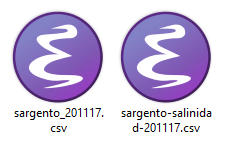
\includegraphics[height=1.9cm]{archivos.png}
\end{center}
El archivo \textit{"sargento\_201117.csv"} contiene 2395 filas de datos en 5 columnas: la primera es "\#" que indica el número de muestra, la segunda es "Date Time" mustra la fecha en GMMt-07:00, la tercera es "Press" medida en kPa, la cuarta es "Temp" medida en $^{\circ}$C y la quinta es "Water Level" medida en m. Mientras que el archivo \textit{"sargento-salinidad-201117.csv"} contiene 2395 filas de datos en 6 columnas:la primera es "\#" que indica el número de muestra, la segunda es "Date Time" mustra la fecha en GMMt-07:00, la tercera es "Cond High"Rng medida en S/cm, la cuarta es "Temp" medida en $^{\circ}$C y la quinta es "Specific Conductance" medida en S/cm y la sexta "Salinity" medida en ppt. En ambos archivos los datos estan tomados cada 15 minutos, para el caso de \textit{"sargento\_201117.csv"} inicia el 26/10/2017 a las 13:00:00 y finaliza el 20/11/2017 a las 11:30:00, por su parte el \textit{"sargento-salinidad-201117.csv"} inicia el 26/10/2017 a las 12:45:00 y finaliza el 20/11/2017 a las 11:15:00.

\subsection*{Anális de Datos}
Primeramente, ya con una vista de la estructura que tiene nuestros archivos se procedió a abrir desde la carpeta Evaluación1 un Jupyter Notebook titulandolo también como Evaluación 1. Inmediatamente en la primera celda se cargaron las bibliotecas correspondientes para inciar el análisis y lectura de datos de los archivos.
\begin{center}
	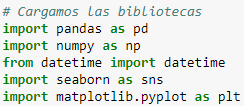
\includegraphics[height=2.5cm]{bibliotecas.png}
\end{center}
Posteriormente se leyeron ambos archivos y se les asignó un data frame, cabe reslatar que en los dos archivos nos saltamos 2 filas (texto basura) y en uno de ellos se ocupó una mas (df2), para que los datos estuieran en "fase" de acuerdo a fecha y hora. Notamos que los datos tampoco finalizaban en "fase" por lo que se eliminó la última fila de un archivo (df1). Parte del texto basura, era el nombre de las columnas por lo que se nombraron de nuevo. Esto se hace para fácilitar la detección del tipo de dato con el que estamos tratando por parte de Pandas.
\begin{center}
	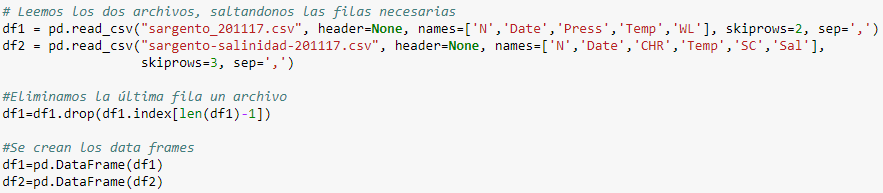
\includegraphics[height=3cm]{lectura.png}
\end{center}
Es importante notar que los nombres de las columnas ahora se encuentan "abreviados".\\

Observamos una muestra de datos para verificar si se estan leyendo correctamente:
\begin{center}
	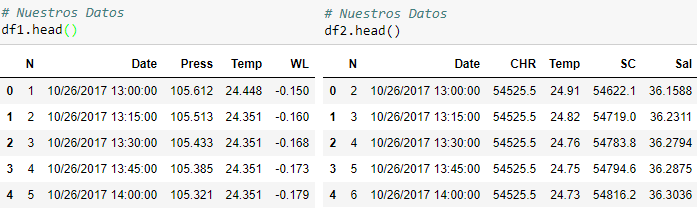
\includegraphics[height=3.5cm]{muestras.png}
\end{center}
Se realizó la conversión de Fecha en formato de fecha, agregando también una columna correspondiente al mes para cada uno de los archivos:
\begin{center}
	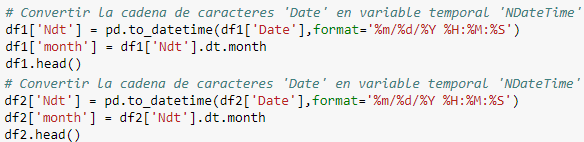
\includegraphics[height=3.5cm]{conversion.png}
\end{center}
\newpage
Verificamos el tipo de datos al que correspondían las variables de cada uno de los archivos:
\begin{center}
	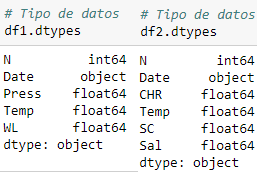
\includegraphics[height=4cm]{tipo.png}
\end{center}
Teniendo todos nuestros datos listos procedimos a crear códigos para realizar las distintas gráficas. Primeramente se nos pidió obtener 3 boxplot con las variables Nivel de Mar, Salinidad y Temperatura de Agua, todo ésto para tener una visualizacion de su variabilidad en el tiempo en que se tomaron los datos. Además con la función describe pudimos saber con exactitud la posición de la mediana, cuarteles, máximos y mínimos.  A continuación semuestras los códigos en el orden de la gráficación de la variables mencionadas:
\begin{center}
	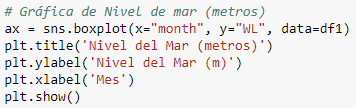
\includegraphics[height=2.4cm]{b1.png}
    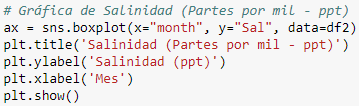
\includegraphics[height=2.4cm]{b2.png}
    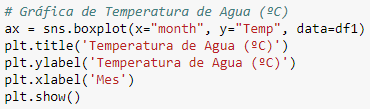
\includegraphics[height=2.4cm]{b3.png}
\end{center}
En la segunda se realizarón Diagramas de Pearson para explorar si hay una correlación de Pearson entre cada pareja de variables (Regresión lineal con las distribuciones marginales): Nivel de mar-Salinidad, Nivel de mar-Temperatura del agua, Salinidad-Temperatura del agua. En el caso de la primera gráfica era necesario crear un nuevo data frame, pues sus variables no corresponden a un solo archivo, si no a los dos, por lo que en el nuevo data frame (df3) juntamos los dos archivos:
\begin{center}
	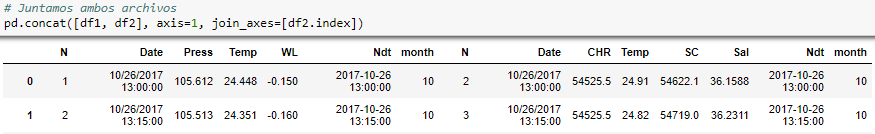
\includegraphics[height=2.5cm]{fusion.png}
\end{center}
Con lo anterior, ya fue posible realizar las gráficas, para las cuales se usaron los siguientes códigos:
\begin{center}
	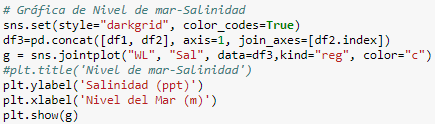
\includegraphics[height=2.8cm]{c1.png}
    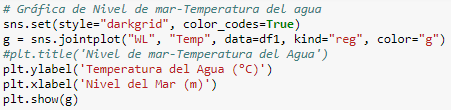
\includegraphics[height=2.4cm]{gc2.png}
    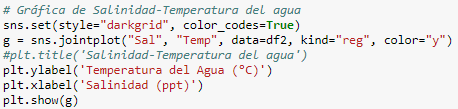
\includegraphics[height=2.34cm]{c3.png}
\end{center}
La tercera parte de gráficas fue de variables en función del tiempo, teniendo nuestras variables Nivel del mar, Salinidad y Temperatura del Agua. Los códigos son los siguientes:
\begin{center}
	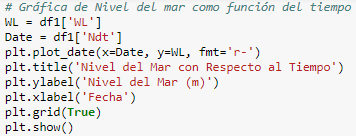
\includegraphics[height=2.9cm]{d1.png}
    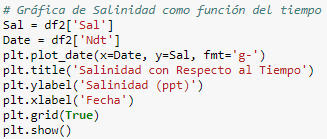
\includegraphics[height=2.9cm]{d2.png}
    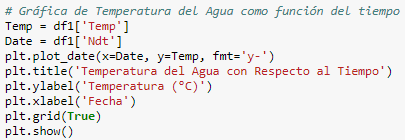
\includegraphics[height=2.9cm]{d3.png}
\end{center}
En una cuarta entrada de gráficas fueron las correspondientes a doble eje (superpuestas), es decir, una variable en la izquierda y otra en la derecha con diferente escala tomando al eje x como el tiempo. Las variables fueron  Nivel de mar y Salinidad; Nivel de mar y Temperatura. A continuación se presenta el código:
\begin{center}
	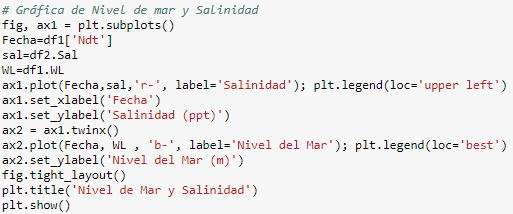
\includegraphics[height=2.9cm]{e1.png}
    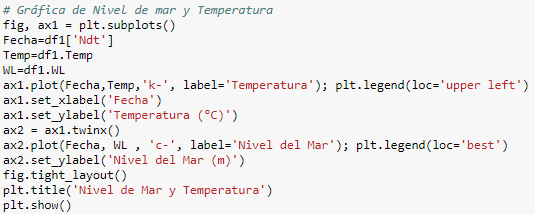
\includegraphics[height=2.9cm]{e2.png}
\end{center}
Para finalizar se nos pidió realizar las mismas gráficas anteriores, pero para un perido de tiempo de 5 días (1-5 de Noviembre) para lo cual tenemos el siguiente código:
\begin{center}
	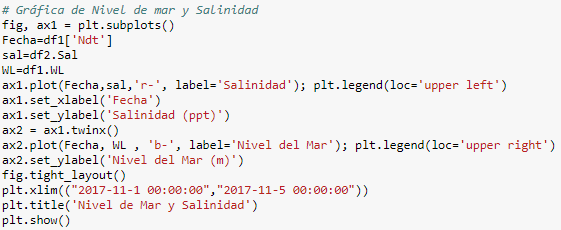
\includegraphics[height=2.9cm]{f1.png}
    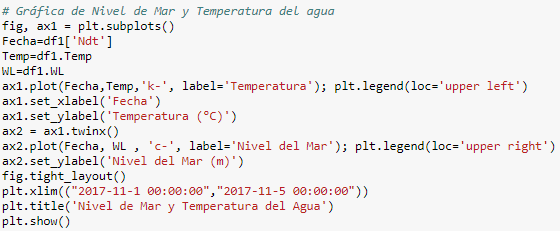
\includegraphics[height=2.9cm]{f2.png}
\end{center}
\section*{Resultados}
Se presentarán las gráficas obtenidas con los segmentos de código anteriores, así como una breve interpretación.
\subsection*{Boxplots}
$\rightarrow$ Nivel del Mar
\begin{center}
	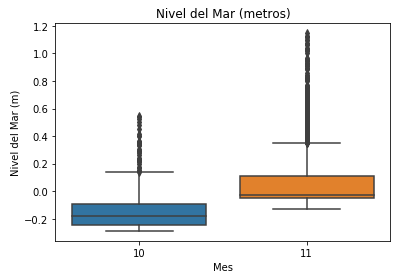
\includegraphics[height=5cm]{gb1.png}
\end{center}
Observamos que existe un aumento de la media de alrededor de 20 cm de octubre a noviembre. También es notable que su distribución es bastante pequeña y que se tiene un aumento considerable del mar pero en centímetros.\\
\newpage
$\rightarrow$ Salinidad
\begin{center}
	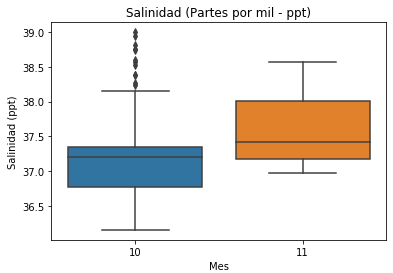
\includegraphics[height=5cm]{gb2.png}
\end{center}
Aunque las cajas de ambos meses tienen una separación considerable, e notorio que la media aparece casi en el mismo valor.\\

$\rightarrow$Temperatura
\begin{center}
	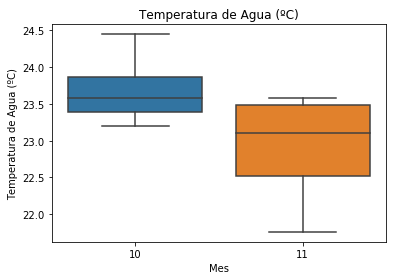
\includegraphics[height=5cm]{gb3.png}
\end{center}
Aquí las temperaturas se encuntran "fijas" por así decirlo, ya que no se muestra un gran cambio considerable.

\subsection*{Describe (función)}
La función permite ver un análisis mas completo de los datos. Aunque en esta ocasión no fue posible encontrar el valor de los cuartiles, máximos, mínimos y mediana que se nos pedían, ya que los datos se clásifican por mes.
\begin{center}
	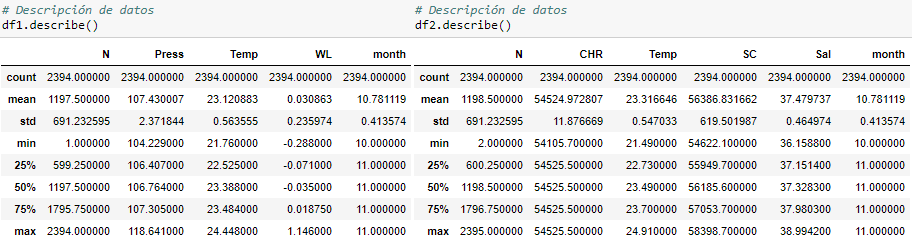
\includegraphics[height=4cm]{descripcion.png}
\end{center}
\subsection*{Diagramas de Pearson}
$\rightarrow$ Salinidad - Nivel del Mar
\begin{center}
	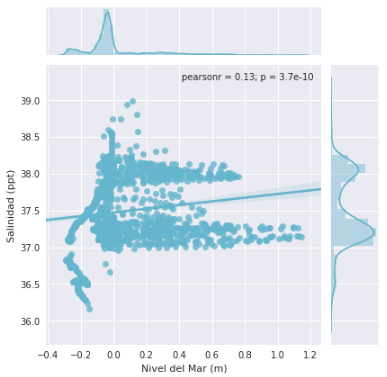
\includegraphics[height=6cm]{gc1.png}
\end{center}
Se puede ver la correlación lineal entre las dos variables, aunque es algo débil. De manera independiente para cada variable, notamos que la salinidad tiene dos picos y el nivel del mar solo uno. \\

$\rightarrow$ Temperatura - Nivel del Mar
\begin{center}
	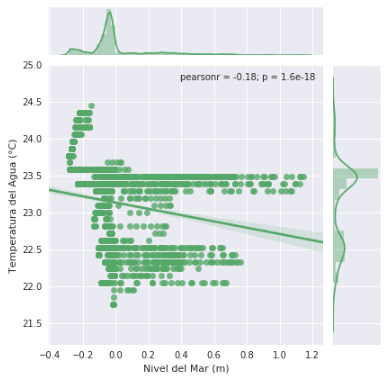
\includegraphics[height=6cm]{gc2_1.png}
\end{center}
Aquí la relación es negativa y al igual que la anterior no es muy fuerte. Aunque si la hay.\\
\newpage
$\rightarrow$ Temperatura - Salinidad
\begin{center}
	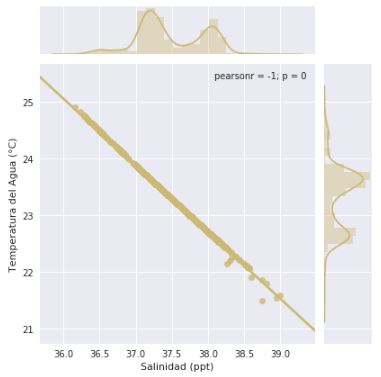
\includegraphics[height=6cm]{gc3.png}
\end{center}
En estas variables si existe un gran correlación lineal negativa, ambas tiene los mismos picos, son bastante similares.

\subsection*{Variables en Función del Tiempo}
$\rightarrow$ Nivel del Mar
\begin{center}
	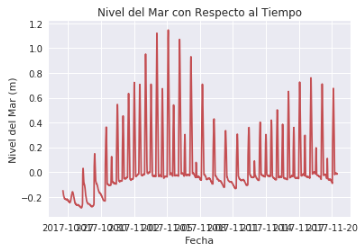
\includegraphics[height=5cm]{gd1.png}
\end{center}
Notamos que conforme pasa el tiempo su comportamiento tiene una distribución de picos, es decir, aumenta y disminuye.\\
\newpage
$\rightarrow$ Salinidad
\begin{center}
	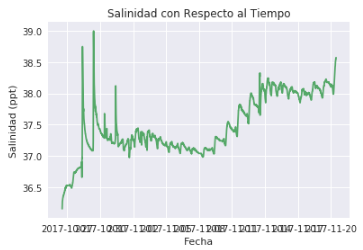
\includegraphics[height=5cm]{gd2.png}
\end{center}
Aunque se cuenta con dos picos, en general esta variable fue incrementanto con el paso del tiempo.\\

$\rightarrow$ Temperatura
\begin{center}
	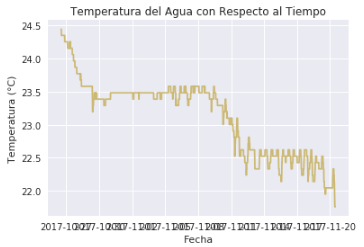
\includegraphics[height=5cm]{gd3.png}
\end{center}
Debido los datos fueron tomados conforme se acercaba el invierno, entonces la temperatura fue disminuyendo.\\

\subsection*{Doble Eje Vertical (Superpuestas)}
$\rightarrow$ Salinidad - Nivel del Mar 
\begin{center}
	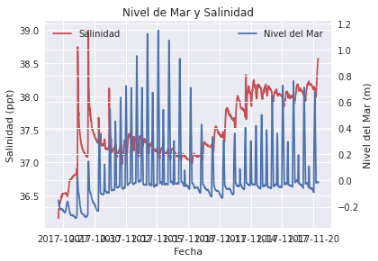
\includegraphics[height=5cm]{ge1.png}
\end{center}
Es observable que las distribuciones no son parecidas, aunque con los diagramas de Pearson concluimos que podria existir cierta relación entre ellas dos.\\

$\rightarrow$ Temperatura - Nivel del Mar
\begin{center}
	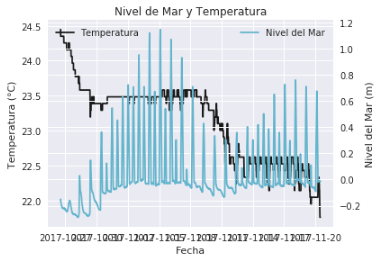
\includegraphics[height=5cm]{ge2.png}
\end{center}
Igual que la anterior, se puede ver que no hay una dependencia o relación entre ambas variables, aunque por el diagrama de Pearson, no es descartable la existencia de una.
\subsection*{Doble Eje Vertical (Superpuestas) en 5 Días}
$\rightarrow$ Salinidad - Nivel del Mar
\begin{center}
	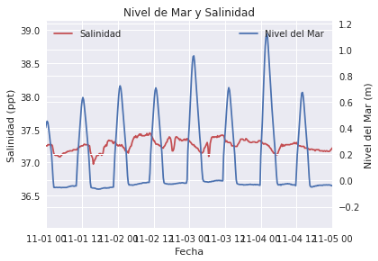
\includegraphics[height=5cm]{gf1.png}
\end{center}
Con el análisis de solo 5 días, es notorio que mientras el nivel del mar aumenta y forma picos (casi periódico), la salinidad podría considerarse como un valor constante. Por lo que no veo que el cambio de una afecte a la otra.\\
\newpage
$\rightarrow$ Temperatura - Nivel del Mar
\begin{center}
	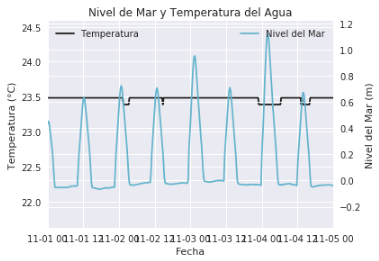
\includegraphics[height=5cm]{gf2.png}
\end{center}
Al igual que la anterior, aquí el nivel del mar tiene un comportamiento aumenta y disminuye (casi periódico) y la temperatura permanece casi constante. Por lo que se podría decir que son variables independientes no importa el cambio de una en la otra.

\section*{Conclusión}
Por último a manera de conclusión se puedo notar una relación muy evidente que es la de la temperatura y la salinidad ya que son inversamente proporcionales (una aumenta y la otra disminuye y visceversa), las otras no están tan relacionadas o al menos no es tan evidente.\\

Por otro lado, la evaluación fue bastante "divertida" aunque fue larga, no era tan complicada ya que solo era poner en práctica lo aprendido y demostrar que éramos capaces de hacerlo y creo que lo logré.

\section*{Bibliografía}
\begin{itemize}
\item Definista. (2018). ¿Qué es Temperatura? - Su Definición, Concepto y Significado. Conceptodefinicion.de. Recuperado el 8 de Marzo de 2018, desde \\
http://conceptodefinicion.de/temperatura/
\item Nivel del mar. (2018). Es.wikipedia.org. Recuperado el 8 de Marzo de 2018, desde 
https://es.wikipedia.org/wiki/Nivel\_del\_mar
\item Salinidad. (2018). Es.wikipedia.org. Recuperado el 8 de Marzo de 2018, desde https://es.wikipedia.org/wiki/Salinidad
\end{itemize}

\end{document}
